\documentclass[aspectratio=169,
				xcolor=table]{beamer}

% Load general definitions
\usepackage[utf8]{inputenc}
%\usepackage[T1]{fontenc}
\usepackage[brazil]{babel}
\usepackage{amsmath}
\usepackage{amsfonts}
\usepackage{amssymb}
\usepackage{graphicx}
\usepackage{verbatim}
\usepackage{cancel}
\usepackage{askmaps}
\usepackage{tabularx}
\usepackage[table]{xcolor}
%\usepackage{tikz}
\usepackage{multirow}
\usepackage{mathtools}
\usepackage{color, colortbl}
\usepackage{etoolbox}
\usepackage{pbox}
\usepackage{changepage}
\usepackage{xpatch}
\usepackage{array}
\usepackage{marvosym}
\usepackage{tabu}
\usepackage{multicol}
\usepackage{listings}
\usepackage{underscore}
\usepackage{filecontents}
\usepackage[]{algorithm2e}
\usepackage{ragged2e}

\newcolumntype{P}[1]{>{\centering\arraybackslash}m{#1}}
\definecolor{Gray}{gray}{0.75}
\definecolor{Gray2}{gray}{0.85}

\definecolor{lightBlue}{HTML}{DAE8FC}
\definecolor{Blue}{RGB}{51, 51, 204}

%\useinnertheme[lily]{rounded}
\usetheme{UniEvangelica}
%\usetheme{Copenhagen}
%\usetheme{Berlin}
%\usecolortheme{dolphin}
\tolerance=1
\emergencystretch=\maxdimen
\hyphenpenalty=10000
\hbadness=10000

\setbeamertemplate{navigation symbols}{}%remove navigation symbols


\let\olditem=\item% 
\renewcommand{\item}{\olditem \justifying}%
\def\center{\trivlist \centering\item\relax}
\def\endcenter{\endtrivlist}

\setbeamertemplate{itemize/enumerate body begin}{\large}
\setbeamertemplate{itemize/enumerate subbody begin}{\large}

\setbeamertemplate{itemize item}{\raisebox{0.1ex}{$\blacktriangleright$}\hskip0.1em}
\setbeamertemplate{itemize subitem}{\raisebox{0.1ex}{$\blacktriangleright$}\hskip0.1em}

\newcommand{\greenarrow}{\textcolor{green}{\rotatebox[origin=c]{180}{\MVArrowDown}}}

\newcommand{\redarrow}{\textcolor{red}{\MVArrowDown}}

%\newcommand{\ftable}{
%	\begin{table}
%		\large
%		\centering
%		\rowcolors{1}{\ifnumless{\rownum}{2}{Blue}{lightBlue}}{}
%}

\newenvironment{eftable}{
	\begin{table}
		\large
		\centering
		\rowcolors{1}{}{Blue}
		\rowcolors{1}{\ifnumless{\rownum}{2}{Blue}{lightBlue}}{}
	}
	{
	\end{table}
}


%\setbeamertemplate{frametitle}
%{
%	%\vspace*{-2em}	
%	\insertframetitle
%
%	 %\textcolor{white}{\LARGE \insertframetitle}
%
%}

% Specific definitions
\institute[]{\uppercase{Engenharia de Software}}
\title[]{Arquitetura e Organização de Computadores}
\subtitle[]{\uppercase{Conceitos Básicos}}
\author[]{Prof. Alexandre Tannus}
\date{}

\begin{document}
	\begin{frame}
		\titlepage
	\end{frame}
	
	\begin{frame}{Objetivos}
		\begin{itemize}
			\item Apresentar os conceitos iniciais de Arquitetura e Organização de Computadores
			\vspace{1em}
			\item Entender o Sistema Internacional de Medidas
			\vspace{1em}
			\item Compreender as diferenças entre o SI e as unidades de medida utilizadas em computação
		\end{itemize}
	\end{frame}
	
%	\begin{frame}{Metodologia}
%		\begin{itemize}
%			\item O tema da aula é exposto pelo professor em sala de aula. Os alunos interagem durante a apresentação para resolução de dúvidas e exposição de questionamentos relevantes ao tema, os quais podem ser sanados diretamente pelo professor ou serem colocados em discussão pela turma. 
%			\vspace{1em}
%			\item Ao final da exposição do conteúdo são resolvidos exercícios de fixação, para melhor compreensão do tema. As questões podem ser retiradas de concursos públicos, ENADE, POSCOMP ou de autoria do próprio professor.
%		\end{itemize}
%	\end{frame}

	\begin{frame}
		\tableofcontents
	\end{frame}	
	
	\section{Introdução}
	\begin{frame}
		\frametitle{Questionamentos}
		\begin{itemize}
			\item O que é arquitetura de computadores?
			\vspace{1em}
			\item O que significa organização de computadores?
			\vspace{1em}
			\item Quais são os componentes fundamentais de um computador e como eles se interconectam?
			\vspace{1em}
			\item Como fazer para comunicar vários computadores?
		\end{itemize}
	\end{frame}
	
	\begin{frame}{Motivação}
		\begin{itemize}
			\item Usuário
			\begin{itemize}
				\item Ciência dos recursos disponíveis, pontos fortes e limitações do sistema computacional
			\end{itemize}
			\vspace{1em}
			\item Programador
			\begin{itemize}
				\item Utilização mais eficaz dos recursos da máquina para otimizar o desempenho dos softwares
			\end{itemize}
		\end{itemize}
	\end{frame}
	
	\begin{frame}
		\frametitle{Motivação}
		\begin{itemize}
			\item Analista de sistemas
			\begin{itemize}
				\item Entendimento das especificações técnicas para embasar a aquisição de equipamentos
				\item Capacidade de analisar a melhor solução para um problema, avaliando as opções disponíveis
			\end{itemize}
			\vspace{1em}
			\item Gerente do sistema
			\begin{itemize}
				\item Entendimento de relatórios de desempenho para maximizar a disponibilidade e eficiência do sistema
			\end{itemize}
		\end{itemize}
	\end{frame}

	\begin{frame}
		\frametitle{Definição}
		\begin{itemize}
			\item Arquitetura
			\begin{itemize}
				\item Atributos visíveis ao programador
				\item Ex.: conjunto de instruções, mecanismos de entrada/saída (E/S), representação de dados
			\end{itemize}
			\vspace{1em}
			\item Organização
			\begin{itemize}
				\item Unidades operacionais e suas interconexões
				\item Ex.: interface computador-periféricos, tecnologia de memória utilizada, detalhes de hardware transparentes ao programador
			\end{itemize}
		\end{itemize}
	\end{frame}
	
	\begin{frame}
		\frametitle{Exemplo - Processadores Intel Core i7}
		\begin{table}
			\Large
				\centering
			\begin{tabular}{l | l}
				\rowcolor{Blue}
				\textcolor{white}{Arquitetura} &
				\textcolor{white}{Modelo (Organização)}\\
				\multirow{5}{*}{7ª geração} & i7-7700 \\
				& \cellcolor{lightBlue}i7-7700K \\
				& i7-7700T \\
				& \cellcolor{lightBlue}i7-7600U \\
				& i7-7500U \\
				\hline
				\cellcolor{lightBlue} & \cellcolor{lightBlue}i7-6700K \\
				\cellcolor{lightBlue}& i7-6700T \\
				\cellcolor{lightBlue}& \cellcolor{lightBlue}i7-6970HQ \\
				\multirow{-4}{*}{\cellcolor{lightBlue}6ª geração}& i7-6500U \\
				\multicolumn{2}{r}{\footnotesize  Fonte: \href{https://goo.gl/Tk0fqA}{\color{blue}{\underline{https://goo.gl/Tk0fqA}}}
}
			\end{tabular}
		\end{table}		
	\end{frame}
	
	\begin{frame}
		\frametitle{Componentes do sistema computacional}
		\begin{itemize}
			\item Hardware
			\begin{itemize}
				\item Parte física do sistema
				\item Componentes eletrônicos, periféricos E/S, etc.
			\end{itemize}
			\vspace{1em}
			\item Software
			\begin{itemize}
				\item Sequência de instruções lógicas
				\item Aplicativos, sistema operacional
			\end{itemize}
		\end{itemize}
	\end{frame}

	\begin{frame}
		\frametitle{Componentes do sistema computacional}
		\begin{itemize}
			\item Dados
			\begin{itemize}
				\item Informação a ser processada e/ou manipulada
				\item Devem ser representados em uma forma reconhecível pelo sistema
			\end{itemize}
			\vspace{1em}
			\item Comunicação
			\begin{itemize}
				\item Possibilita a conexão entre sistemas
			\end{itemize}
		\end{itemize}
	\end{frame}
	
	\begin{frame}
		\frametitle{Modelo Hierárquico}
		\begin{itemize}
			\item Define níveis com um conjunto de componentes e seus respectivos inter-relacionamentos
			\vspace{1em}
			\item Em cada nível é importante reconhecer a estrutura e a função
			\begin{itemize}
				\item Estrutura: como os componentes são inter-relacionados
				\item Função: operação individual de cada componente
			\end{itemize}
			\vspace{1em}			
			\item Facilita a compreensão e projeto do sistema

		\end{itemize}
	\end{frame}

	\begin{frame}
		\frametitle{Modelo hierárquico - exemplo}
		\begin{figure}
			\centering
			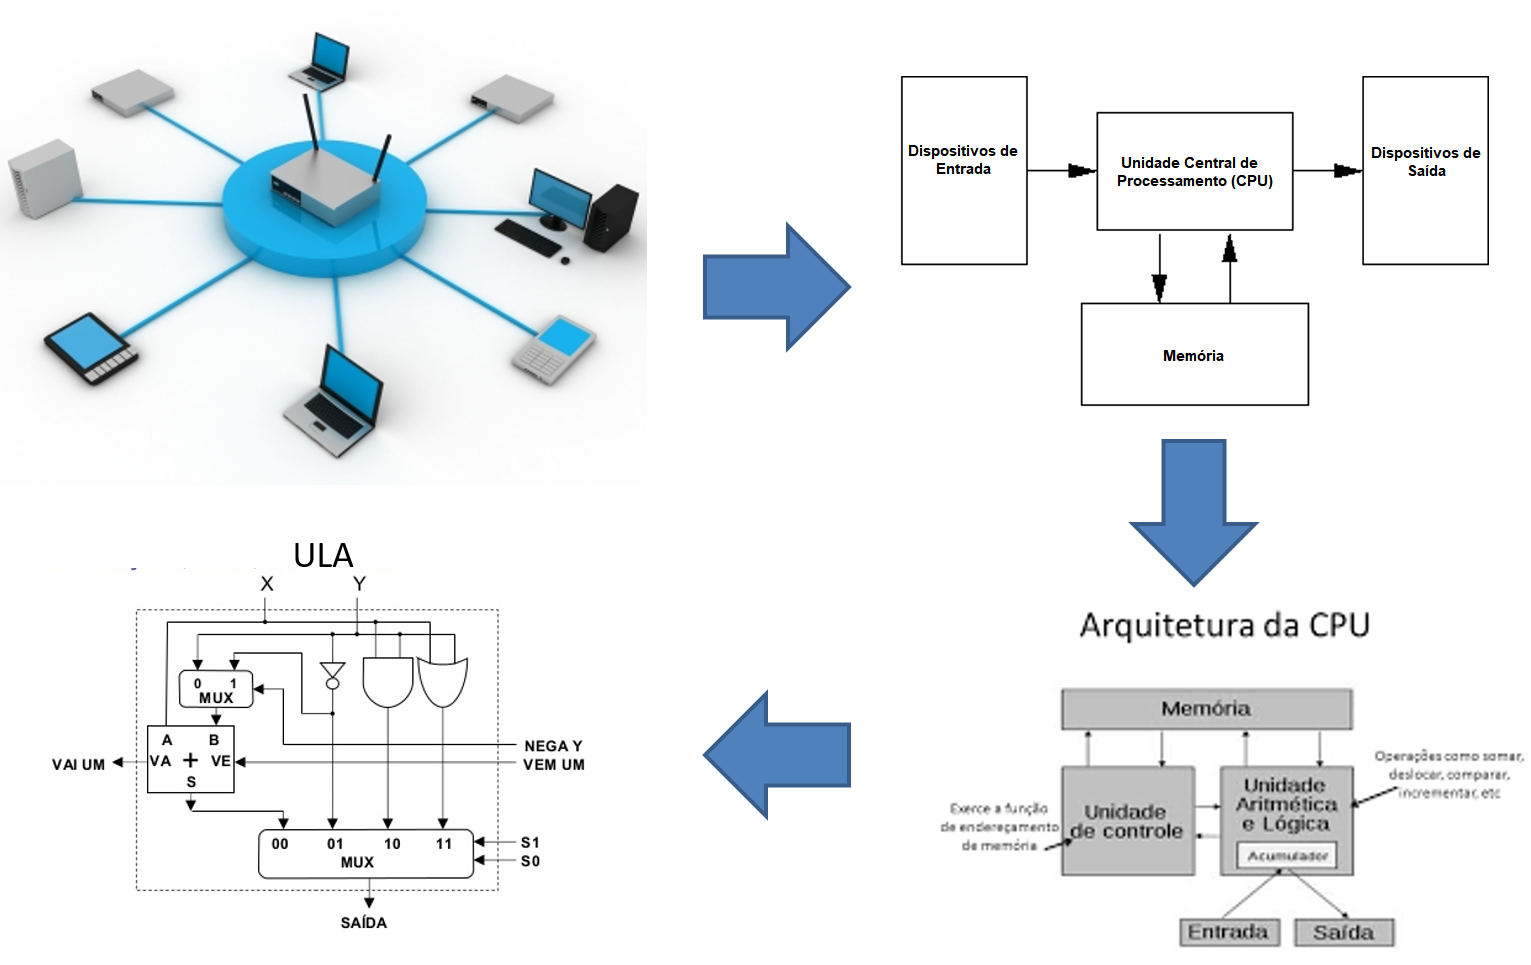
\includegraphics[height=6cm, keepaspectratio]{../figs/cap01/hierarquia.png} 
		\end{figure}
	\end{frame}

	\begin{frame}
		\frametitle{Modelo hierárquico - exemplo}
		\begin{figure}
			\centering
			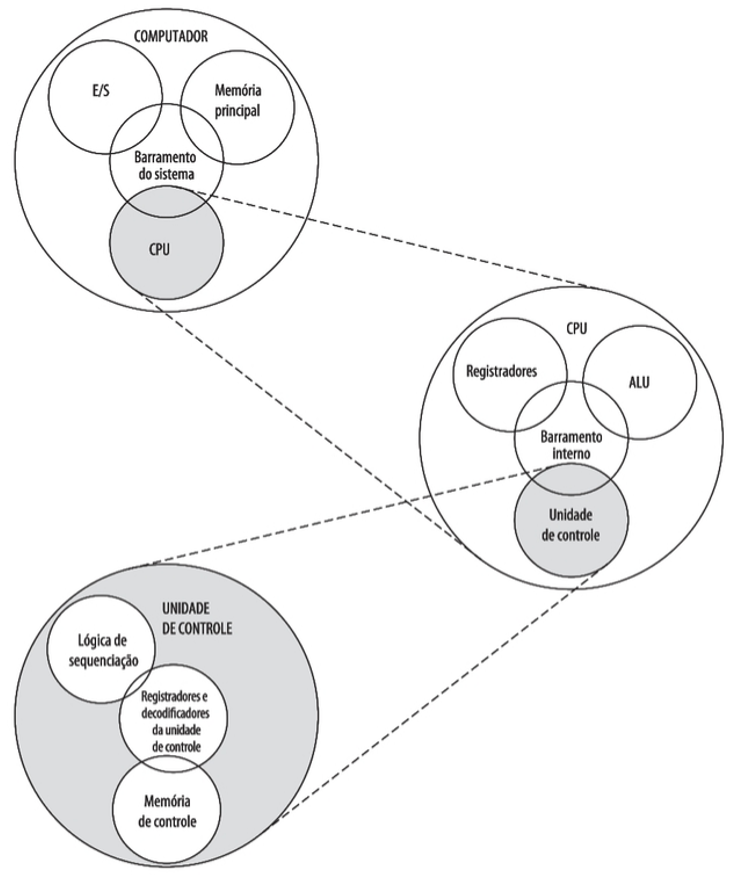
\includegraphics[height=6cm, keepaspectratio]{../figs/cap01/hierarquia2.png} 
		\end{figure}
	\end{frame}
	
	\begin{frame}
		\frametitle{Funções do sistema computacional}
		\begin{itemize}
			\item Processamento de dados

			\item Armazenamento de dados

			\item Movimentação de dados
			\begin{itemize}
				\item Entrada (\textit{Input}) e saída (\textit{Output})
			\end{itemize}

			\item Controle

		\end{itemize}
	\end{frame}	

	\begin{frame}
		\frametitle{Estrutura}
		\begin{columns}
			\begin{column}{0.65\textwidth}
			\begin{itemize}
				\item Unidade Central de Processamento (CPU)

				\item Memória

				\item Dispositivos de Entrada/Saída

				\item Barramentos

			\end{itemize}
			\end{column}
			\begin{column}{0.35\textwidth}
				\begin{figure}
					\centering
					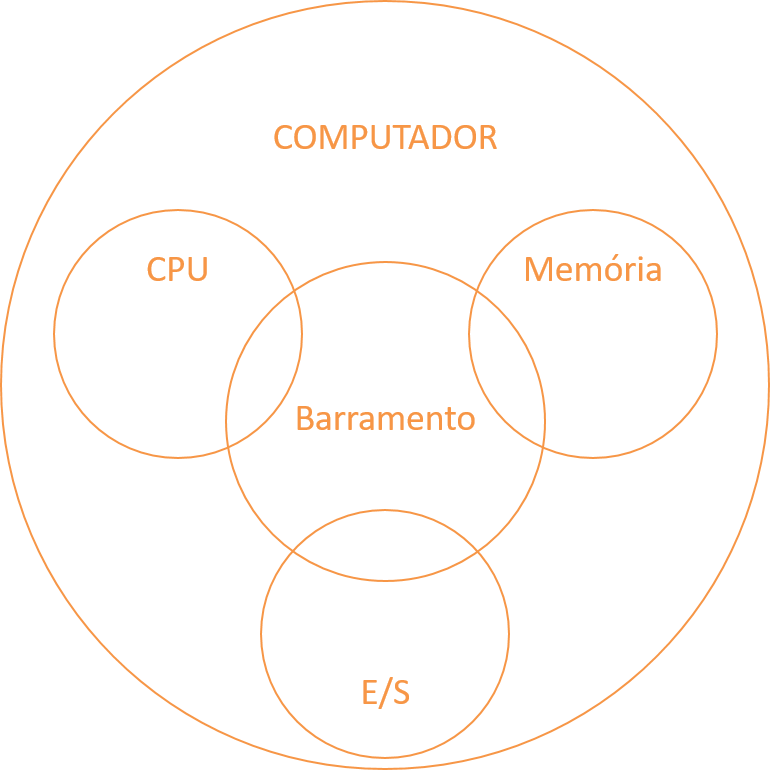
\includegraphics[width=0.9\textwidth, keepaspectratio]{../figs/cap01/cpu.png} 
				\end{figure}
			\end{column}
		\end{columns}
	\end{frame}
	
	\begin{frame}
		\frametitle{Padrões e protocolos}
		\begin{columns}
			\begin{column}{0.63\textwidth}
				\begin{itemize}
					\item Padrões
					\begin{itemize}
						\item Garantem o funcionamento em conjunto de diversos componentes do sistema, mesmo que sejam de fabricantes diferentes
						\item Aplicáveis ao hardware, software, dados e comunicação
		
					\end{itemize}
				\end{itemize}

			\end{column}
			\begin{column}{0.37\textwidth}
			\begin{itemize}
				\item Exemplos
				\begin{itemize}
					\item Hardware:  tensão de alimentação, pinos de um conector
					\item Software: SQL, máquinas virtuais
					\item Dados: JPEG, GIF, PDF
					\item Comunicação: Ethernet

				\end{itemize}
			\end{itemize}
			\end{column}
		\end{columns}
	\end{frame}	

	\section{Conceitos Importantes}
	\begin{frame}
		\frametitle{Padrões e protocolos}
		\begin{columns}
			\begin{column}{0.55\textwidth}
				\begin{itemize}
					\item Protocolos
					\begin{itemize}
						\item Conjuntos específicos de regras básicas acordadas que possibilitam a comunicação (Englander, 2011)

					\end{itemize}
				\end{itemize}
			\end{column}
			\begin{column}{0.45\textwidth}
				\begin{itemize}
					\item Exemplos
					\begin{itemize}
						\item HTTP
						\item TCP/IP
					\end{itemize}
				\end{itemize}
			\end{column}
		\end{columns}
	\end{frame}
	
	\begin{frame}
		\frametitle{Firmware}
		\begin{itemize}
			\item Conjunto de instruções desenvolvido para realizar o gerenciamento do hardware em um dispositivo eletrônico
			\vspace{1em}
			\item Depende totalmente da arquitetura do dispositivo
			\vspace{1em}
			\item Ex.: BIOS
		\end{itemize}
	\end{frame}
	
	\begin{frame}
		\frametitle{Sistema operacional}
		\begin{itemize}
			\item Software responsável pela interpretação de comandos e interface usuário-máquina
			\vspace{1em}
			\item Realiza o gerenciamento dos aplicativos executados pelo usuário
			\vspace{1em}
			\item Ex.: Windows, Linux, iOS, Android
		\end{itemize}
	\end{frame}

	\begin{frame}
		\frametitle{Linguagem de máquina}
		\begin{columns}
			\begin{column}{0.55\textwidth}
				\begin{itemize}
					\item Sequência ordenada de números que representam as instruções que serão executadas pelo processador
					\vspace{1em}
					\item Cada processador possui um conjunto específico de instruções
				\end{itemize}
			\end{column}
			\begin{column}{0.45\textwidth}
			\begin{figure}
				\centering
				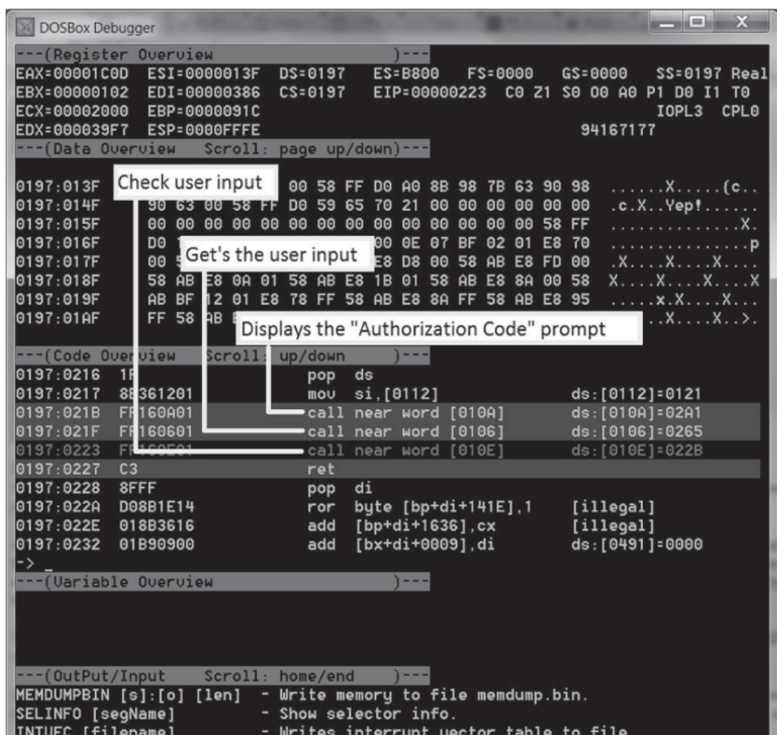
\includegraphics[width=0.9\textwidth, keepaspectratio]{../figs/cap01/linguagemMaquina.png} 
			\end{figure}
			\end{column}
		\end{columns}
	\end{frame}
	
	\section{Sistemas de medidas}
	
	\begin{frame}
		\frametitle{Sistema Internacional}
		\begin{eftable}
			\Large
			\begin{tabular}{l | c | c}
			\textcolor{white}{Medida} &
			\textcolor{white}{Unidade} &
			\textcolor{white}{Símbolo} \\
			Comprimento & metro & m \\
			Tempo & segundo & s \\
			Massa & grama & g \\
			Velocidade & metro por segundo & m/s \\
			Resistência elétrica & Ohm & $\Omega$ \\
			Tensão elétrica & Volt & V \\
			Corrente elétrica & Ampere & A \\
			Frequência & Hertz & Hz
			
			
			\end{tabular}
		\end{eftable}
	\end{frame}
	
	\begin{frame}
		\frametitle{Sistema Internacional - Submúltiplos}
		\begin{eftable}
			\Large
			\begin{tabular}{c | c | c | l}
				\textcolor{white}{Prefixo} &
				\textcolor{white}{Símbolo} &				
				\textcolor{white}{Expoente} &
				\textcolor{white}{Explícito} \\
				mili  & m & $10^{-3}$  & $0,001$ \\
				micro &  $\mu$ & $10^{-6}$  & $0,000001$ \\
				nano  & n & $10^{-9}$  & $0,000000001$ \\
				pico  & p & $10^{-12}$ & $0,000000000001$ \\
				femto & f & $10^{-15}$ & $0,000000000000001$ \\				
			\end{tabular}
		\end{eftable}
	\end{frame}

	\begin{frame}
		\frametitle{Sistema Internacional - Múltiplos}
		\begin{eftable}
			\Large
			\begin{tabular}{c | c | c | l}
				\textcolor{white}{Prefixo} &
				\textcolor{white}{Símbolo} &
				\textcolor{white}{Expoente} &
				\textcolor{white}{Explícito} \\
				kilo & k & $10^{3}$  & $1.000$ \\
				mega & M & $10^{6}$  & $1.000.000$ \\
				giga & G & $10^{9}$  & $1.000.000.000$ \\
				tera & T & $10^{12}$ & $1.000.000.000.000$ \\
				peta & P & $10^{15}$ & $1.000.000.000.000.000$ \\
			\end{tabular}
		\end{eftable}
	\end{frame}
	
	\begin{frame}
		\frametitle{Sistema de Medidas em Computação}
		\begin{itemize}
			\item Unidade Fundamental - bit	
			\item Múltiplos do bit					
		\end{itemize}
		\begin{eftable}
			\Large
			\begin{tabular}{c | c}
				\textcolor{white}{Unidade} & 
				\textcolor{white}{Tamanho} \\
				\textit{nibble} & 4 bits \\
				\textit{byte} & 8 bits \\
				\textit{word} & 16 bits \\
				\textit{long word} & 32 bits
			\end{tabular}
		\end{eftable}
	\end{frame}
	
	\begin{frame}	
		\frametitle{Sistema de Medidas em Computação - Múltiplos}
		\begin{eftable}
			\Large
			\begin{tabular}{c | c | l}
				\textcolor{white}{Prefixo} &
				\textcolor{white}{Expoente} &
				\textcolor{white}{Explícito} \\
				kilo & $2^{10}$ & $1.024$ \\
				mega & $2^{20}$ & $1.048.576$ \\
				giga & $2^{30}$ & $1.073.741.824$ \\
				tera & $2^{40}$ & $1.099.511.627.776$ \\
				peta & $2^{50}$ & $1.125.899.906.842.624$ \\
			\end{tabular}
		\end{eftable}
	\end{frame}

	\section{Exercícios}
	
	\begin{frame}{Questão 1 - Prefeitura de João Pessoa - PB 2018}
		Qual é o nome da menor unidade de dado em um sistema computacional?
		\begin{enumerate}[A]
			\item Byte.
			\item Arquivo.
			\item Bit.
			\item ASCII.
		\end{enumerate}

	\end{frame}

	\begin{frame}{Questão 2 - Câmara Municipal de Paraíso do Norte - PR 2018}
		Marque a alternativa abaixo que corresponde a equivalência de 1024 kilobytes (KB).
		\begin{enumerate}[A]
			\item 1 TB
			\item 1 MB
			\item 1 GB
			\item 1 KB
			\item 2 KB
		\end{enumerate}
	\end{frame}

	\begin{frame}{Questão 3 - CRA-SC 2017}
		Assinale a alternativa que indique corretamente a quantidade de bit correspondente a 1KB: 
		\begin{enumerate}[A]
			\item 1024 MB 
			\item 1024 bits 
			\item 1000 bits 
			\item 246 GB 
		\end{enumerate}		
	\end{frame}
	
	\begin{frame}{Questão 4 - CRA-SC 2017}
		Assinale a alternativa correta. 
		\begin{enumerate}[A]
			\item CPU é um mnemônico que significa Centro de Processamento Unitário. 
			\item A unidade básica da informação é o digito.
			\item KiloByte, GigaByte e MegaByte são tipos de arquivo. 
			\item 1 Byte tem 8 bits e 1KB tem 1024 bits. 
		\end{enumerate}
	\end{frame}

	\begin{frame}{Questão 5 - CAU-MG 2014}
		Em relação à organização dos sistemas computacionais, as alternativas abaixo apresentam os principais componentes, EXCETO: 
		\begin{enumerate}[A]
			\item Componentes de E/S.
			\item Sistema operacional.
			\item Memória.
			\item Processador. 
		\end{enumerate}
	\end{frame}
	
	\begin{frame}{Questão 6 - CEGÁS 2017}
		O programa que analisa e traduz um código de alto nível, para a linguagem do computador (máquina) e que roda o código-fonte escrito como sendo o código objeto, traduzindo o programa linha a linha, sendo que o programa vai sendo utilizado na medida em que vai sendo traduzido, é denominado de:  
		\begin{enumerate}[A]
			\item Editor de texto.
			\item Interpretador. 
			\item Compilador.  
			\item Depurador.
		\end{enumerate}
	\end{frame}
	
	\begin{frame}[allowframebreaks]{Questão 7 -  TJ-PR 2013}
		Sobre conceitos de informática, considere as seguintes afirmativas:  
		\begin{enumerate}
			\item Hardware é um conjunto de protocolos, memória principal e componentes eletrônicos com os quais são construídos os computadores e equipamentos periféricos. 
			\item Software é um conjunto de programas, procedimentos e documentação que permitem usufruir da capacidade de processamento fornecida pelo hardware. 
			\item Memória Principal é um conjunto de circuitos de apoio ao processador presentes numa placa-mãe, cuja qualidade influi diretamente na qualidade e no desempenho do computador. 
			\item Programa é um roteiro que orienta o computador, mostrando-lhe a sequência de operações necessárias para executar uma determinada tarefa.  
Assinale a alternativa correta.
		\end{enumerate}
		\framebreak
		\begin{enumerate}[A]
			\item Somente a afirmativa 1 é verdadeira.
			\item Somente as afirmativas 1 e 3 são verdadeiras. 
			\item Somente as afirmativas 2 e 4 são verdadeiras.
			\item Somente as afirmativas 2, 3 e 4 são verdadeiras.
		\end{enumerate}
	\end{frame}
	
	\begin{frame}{Questão 8 - EBSERH 2017}
		Preencha, adequadamente, as especificações encontradas atualmente em um site de vendas de microcomputadores preenchendo as lacunas com as unidades corretas:
		\vspace{0.5em}
		\begin{table}
			\centering
			\begin{tabular}{|ll|}
			\hline 
			FONTE DE ALIMENTAÇÃO & 350 ____ \\ 
			\hline 
			PROCESSADOR AMD FX-3600 & 3.5 ____ \\ 
			\hline 
			HD & 1 ____ e 7200 ____ \\ 
			\hline 
			\end{tabular}		
		\end{table}
 
		
		\vspace{0.5em}
		Assinale a alternativa que apresenta a sequência correta de cima para baixo. 
		\vspace{0.5em}
		\begin{enumerate}[A]
			\item kW - GHz - TB e RPM
			\item W - GHz - GB e RPH
			\item W - GB - TB e RPH
			\item W - GHz - TB e RPM
			\item kW - GB - kB e RPM
		\end{enumerate}

	\end{frame}

	\begin{frame}[allowframebreaks]{Questão 9 - UFAL 2016}
		Considere as afirmativas:
		
		\begin{enumerate}[I]
			\item cria o código objeto traduzindo as instruções da linguagem de montagem (assembly) para código de máquina;
			\item recebe como entrada um conjunto de arquivos objetos e bibliotecas, e produz como resultado um arquivo objeto de saída;
			\item traduz um programa descrito em uma linguagem de alto nível para um programa em linguagem simbólica ou linguagem de máquina;
			\item recebe uma instrução do programa fonte, converte-a em linguagem de máquina e ordena ao computador que execute esta instrução.

		\end{enumerate}
		\framebreak
		Nessa ordem, os itens de I a IV referem-se a  
		\begin{enumerate}[A]
			\item ligador, montador, interpretador e montador.  
			\item ligador, montador, compilador e interpretador.  
			\item interpretador, ligador, compilador e montador.  
			\item montador, ligador, compilador e interpretador.  
			\item compilador, ligador, montador e interpretador. 
		\end{enumerate}
	\end{frame}

	\begin{frame}{Questão 10 - Câmara Municipal de Caruaru - PE 2015}
		O número de valores que uma palavra de 16 bits pode representar é 
		\begin{itemize}
			\item 16384
			\item 32768
			\item 65536
			\item 262144
			\item 1048576 
		\end{itemize}

	\end{frame}
	
	\begin{frame}{Respostas}
		1 - B \\
		2 - C \\
		3 - B \\
		4 - D \\
		5 - B \\
		6 - B \\
		7 - C \\
		8 - D \\
		9 - D \\
		10 - C
	\end{frame}
	
	\begin{frame}{Bibliografia}
		\nocite{Englander2011}
		\nocite{Paixao2014}
		\nocite{Stallings2010}
    	\bibliographystyle{plain}
    	\bibliography{../refs}   	
	
	\end{frame}
	
	\begin{frame}{}
			
		\end{frame}	
\end{document}